\documentclass{standalone}
\usepackage{tikz}
\usetikzlibrary{patterns, positioning}
\usepackage[sfdefault]{ClearSans} %% option 'sfdefault' activates Clear Sans as the default text font
\usepackage[T1]{fontenc}

\begin{document}
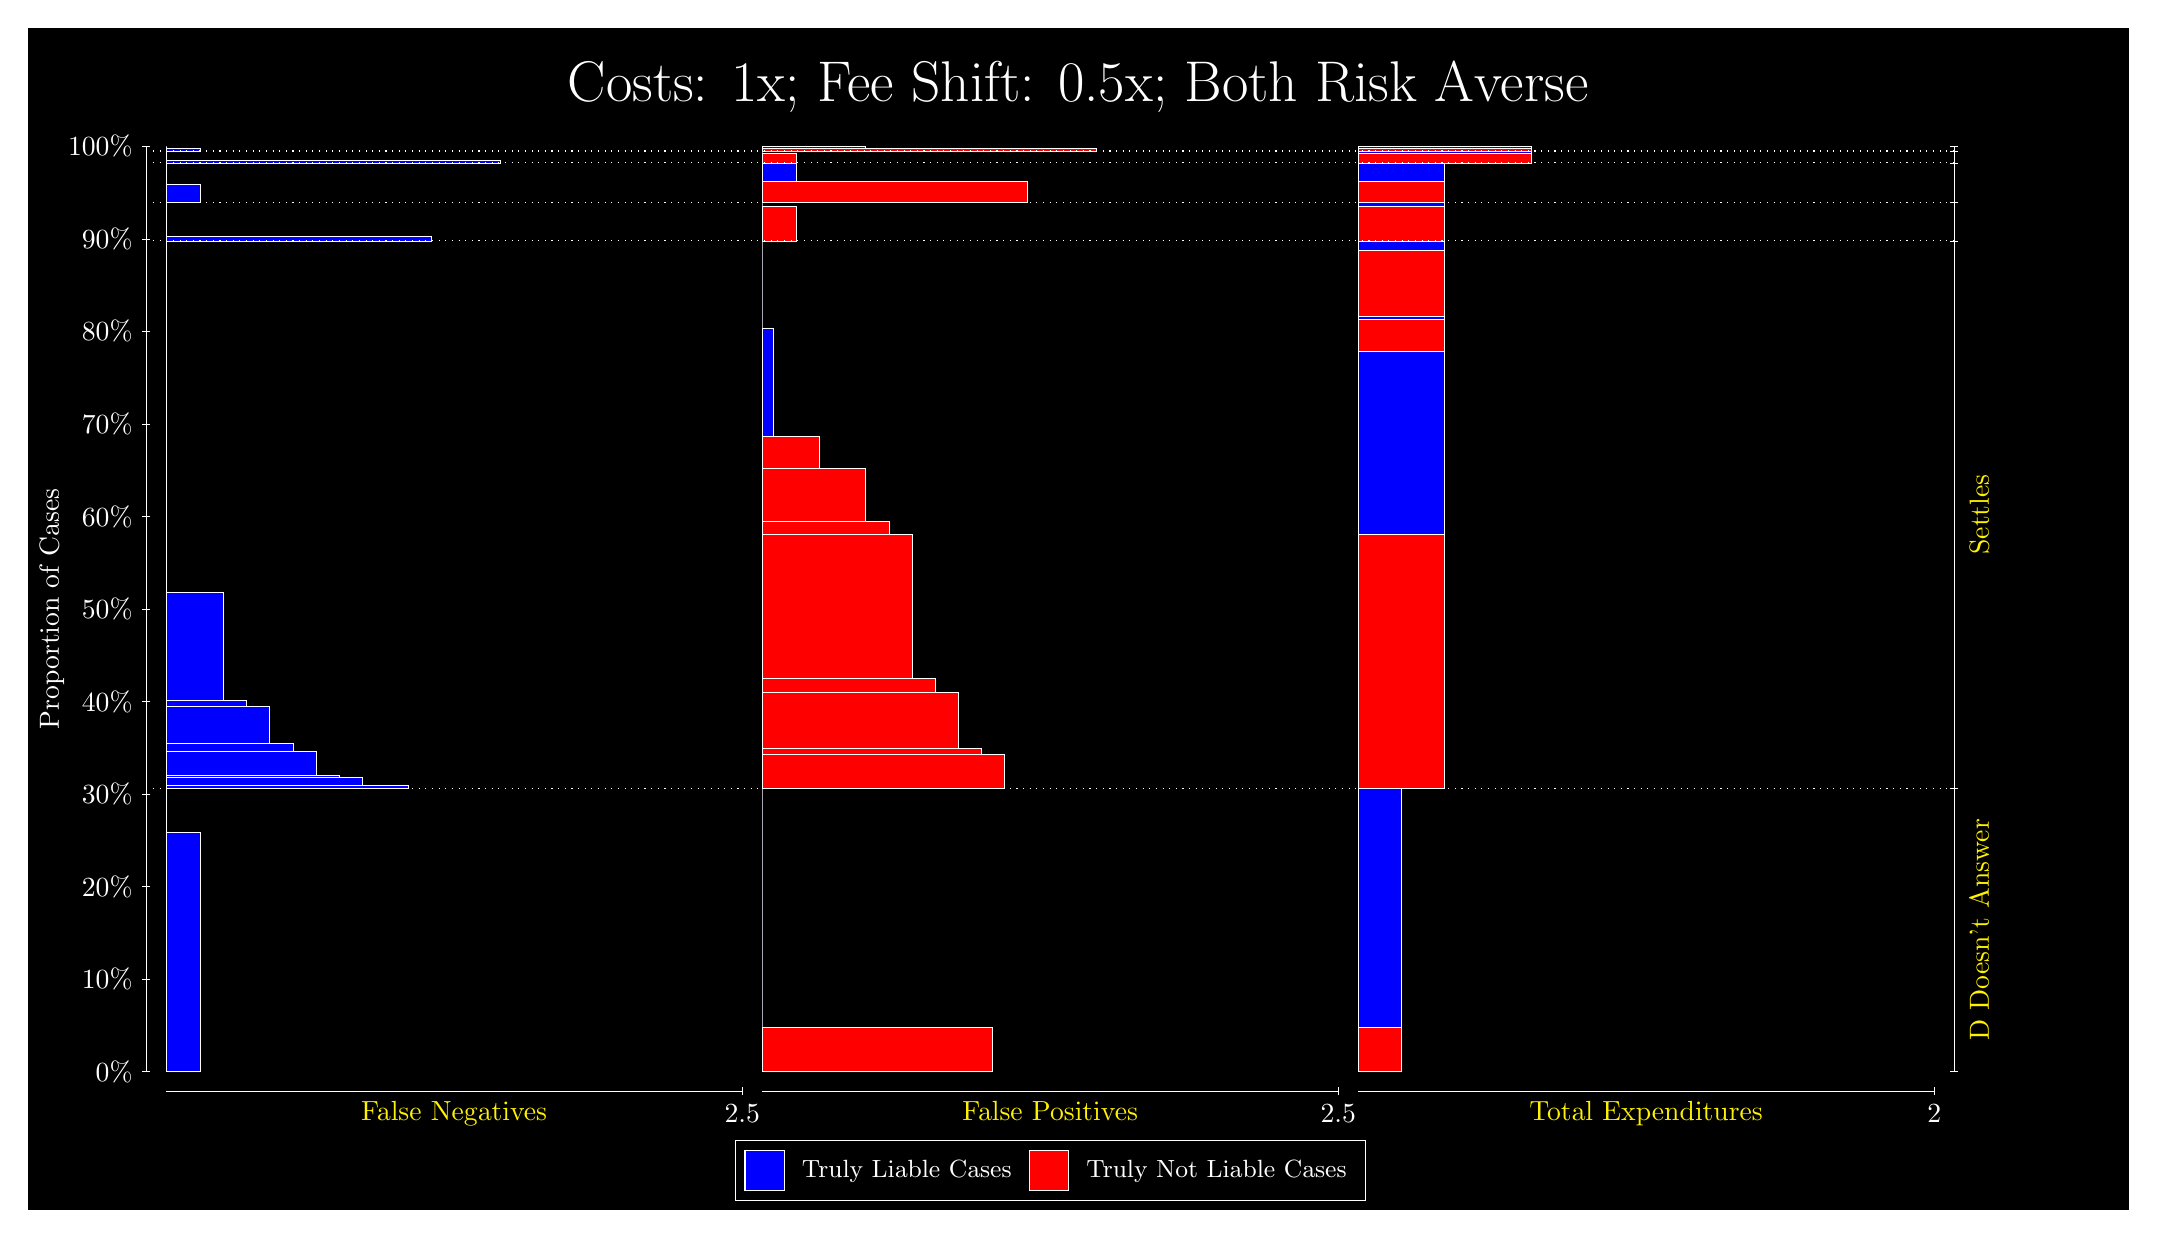
\begin{tikzpicture}
\draw[fill=black] (0,0) rectangle (26.667,15);
\draw[text=white] (0,13.5) rectangle (26.667,15) node[midway] {\huge Costs: 1x; Fee Shift: 0.5x; Both Risk Averse};
\draw[white, very thin] (1.5,1.75) -- (1.5,13.5);
\node[rotate=90, text=white, anchor=center] at (0.3, 7.625) {Proportion of Cases};
\draw[white, very thin] (1.45,1.75) -- (1.55,1.75);
\node[text=white, anchor=east] at (1.45, 1.75) {0\%};
\draw[white, very thin] (1.45,2.925) -- (1.55,2.925);
\node[text=white, anchor=east] at (1.45, 2.925) {10\%};
\draw[white, very thin] (1.45,4.1) -- (1.55,4.1);
\node[text=white, anchor=east] at (1.45, 4.1) {20\%};
\draw[white, very thin] (1.45,5.275) -- (1.55,5.275);
\node[text=white, anchor=east] at (1.45, 5.275) {30\%};
\draw[white, very thin] (1.45,6.45) -- (1.55,6.45);
\node[text=white, anchor=east] at (1.45, 6.45) {40\%};
\draw[white, very thin] (1.45,7.625) -- (1.55,7.625);
\node[text=white, anchor=east] at (1.45, 7.625) {50\%};
\draw[white, very thin] (1.45,8.8) -- (1.55,8.8);
\node[text=white, anchor=east] at (1.45, 8.8) {60\%};
\draw[white, very thin] (1.45,9.975) -- (1.55,9.975);
\node[text=white, anchor=east] at (1.45, 9.975) {70\%};
\draw[white, very thin] (1.45,11.15) -- (1.55,11.15);
\node[text=white, anchor=east] at (1.45, 11.15) {80\%};
\draw[white, very thin] (1.45,12.325) -- (1.55,12.325);
\node[text=white, anchor=east] at (1.45, 12.325) {90\%};
\draw[white, very thin] (1.45,13.5) -- (1.55,13.5);
\node[text=white, anchor=east] at (1.45, 13.5) {100\%};

\draw[white, very thin] (24.457,1.75) -- (24.457,13.5);
\draw[white, very thin] (24.407,1.75) -- (24.507,1.75);
\node[anchor=west] at (24.407, 1.75) {};
\draw[white, very thin] (24.407,5.3476) -- (24.507,5.3476);
\node[anchor=west] at (24.407, 5.3476) {};
\draw[white, very thin] (24.407,12.3) -- (24.507,12.3);
\node[anchor=west] at (24.407, 12.3) {};
\draw[white, very thin] (24.407,12.792) -- (24.507,12.792);
\node[anchor=west] at (24.407, 12.792) {};
\draw[white, very thin] (24.407,13.29) -- (24.507,13.29);
\node[anchor=west] at (24.407, 13.29) {};
\draw[white, very thin] (24.407,13.44) -- (24.507,13.44);
\node[anchor=west] at (24.407, 13.44) {};
\draw[white, very thin] (24.407,13.5) -- (24.507,13.5);
\node[anchor=west] at (24.407, 13.5) {};

\draw[white, very thin, fill=blue] (1.75,1.75) rectangle (2.1891,4.7919);
\draw[white, very thin, fill=red] (1.75,4.7919) rectangle (1.75,5.3476);
\draw[white, very thin, fill=blue] (1.75,5.3476) rectangle (4.8239,5.3879);
\draw[white, very thin, fill=blue] (1.75,5.3879) rectangle (4.2384,5.4852);
\draw[white, very thin, fill=blue] (1.75,5.4852) rectangle (3.9457,5.5107);
\draw[white, very thin, fill=blue] (1.75,5.5107) rectangle (3.6529,5.8219);
\draw[white, very thin, fill=blue] (1.75,5.8219) rectangle (3.3602,5.9158);
\draw[white, very thin, fill=blue] (1.75,5.9158) rectangle (3.0674,6.393);
\draw[white, very thin, fill=blue] (1.75,6.393) rectangle (2.7746,6.4612);
\draw[white, very thin, fill=blue] (1.75,6.4612) rectangle (2.4819,7.8356);
\draw[white, very thin, fill=red] (1.75,7.8356) rectangle (1.75,12.3);
\draw[white, very thin, fill=blue] (1.75,12.3) rectangle (5.1167,12.356);
\draw[white, very thin, fill=red] (1.75,12.356) rectangle (1.75,12.792);
\draw[white, very thin, fill=blue] (1.75,12.792) rectangle (2.1891,13.021);
\draw[white, very thin, fill=red] (1.75,13.021) rectangle (1.75,13.29);
\draw[white, very thin, fill=blue] (1.75,13.29) rectangle (5.9949,13.32);
\draw[white, very thin, fill=red] (1.75,13.32) rectangle (1.75,13.44);
\draw[white, very thin, fill=blue] (1.75,13.44) rectangle (2.1891,13.47);
\draw[white, very thin, fill=red] (1.75,13.47) rectangle (1.75,13.5);
\draw[white, very thin, fill=red] (9.3189,1.75) rectangle (12.246,2.3057);
\draw[white, very thin, fill=blue] (9.3189,2.3057) rectangle (9.3189,5.3476);
\draw[white, very thin, fill=red] (9.3189,5.3476) rectangle (12.393,5.782);
\draw[white, very thin, fill=red] (9.3189,5.782) rectangle (12.1,5.8556);
\draw[white, very thin, fill=red] (9.3189,5.8556) rectangle (11.807,6.5671);
\draw[white, very thin, fill=red] (9.3189,6.5671) rectangle (11.515,6.7423);
\draw[white, very thin, fill=red] (9.3189,6.7423) rectangle (11.222,8.5732);
\draw[white, very thin, fill=red] (9.3189,8.5732) rectangle (10.929,8.7378);
\draw[white, very thin, fill=red] (9.3189,8.7378) rectangle (10.636,9.4125);
\draw[white, very thin, fill=red] (9.3189,9.4125) rectangle (10.051,9.8124);
\draw[white, very thin, fill=blue] (9.3189,9.8124) rectangle (9.4652,11.187);
\draw[white, very thin, fill=blue] (9.3189,11.187) rectangle (9.3189,12.3);
\draw[white, very thin, fill=red] (9.3189,12.3) rectangle (9.758,12.736);
\draw[white, very thin, fill=blue] (9.3189,12.736) rectangle (9.3189,12.792);
\draw[white, very thin, fill=red] (9.3189,12.792) rectangle (12.686,13.061);
\draw[white, very thin, fill=blue] (9.3189,13.061) rectangle (9.758,13.29);
\draw[white, very thin, fill=red] (9.3189,13.29) rectangle (9.758,13.41);
\draw[white, very thin, fill=blue] (9.3189,13.41) rectangle (9.3189,13.44);
\draw[white, very thin, fill=red] (9.3189,13.44) rectangle (13.564,13.47);
\draw[white, very thin, fill=blue] (9.3189,13.47) rectangle (10.636,13.5);
\draw[white, very thin, fill=red] (16.888,1.75) rectangle (17.437,2.3057);
\draw[white, very thin, fill=blue] (16.888,2.3057) rectangle (17.437,5.3476);
\draw[white, very thin, fill=red] (16.888,5.3476) rectangle (17.986,8.5732);
\draw[white, very thin, fill=blue] (16.888,8.5732) rectangle (17.986,10.898);
\draw[white, very thin, fill=red] (16.888,10.898) rectangle (17.986,11.298);
\draw[white, very thin, fill=blue] (16.888,11.298) rectangle (17.986,11.338);
\draw[white, very thin, fill=red] (16.888,11.338) rectangle (17.986,12.178);
\draw[white, very thin, fill=blue] (16.888,12.178) rectangle (17.986,12.3);
\draw[white, very thin, fill=red] (16.888,12.3) rectangle (17.986,12.736);
\draw[white, very thin, fill=blue] (16.888,12.736) rectangle (17.986,12.792);
\draw[white, very thin, fill=red] (16.888,12.792) rectangle (17.986,13.061);
\draw[white, very thin, fill=blue] (16.888,13.061) rectangle (17.986,13.29);
\draw[white, very thin, fill=red] (16.888,13.29) rectangle (19.083,13.41);
\draw[white, very thin, fill=blue] (16.888,13.41) rectangle (19.083,13.44);
\draw[white, very thin, fill=red] (16.888,13.44) rectangle (19.083,13.47);
\draw[white, very thin, fill=blue] (16.888,13.47) rectangle (19.083,13.5);
\draw[white, dotted] (1.5,5.3476) -- (24.457,5.3476);
\draw[white, dotted] (1.5,12.3) -- (24.457,12.3);
\draw[white, dotted] (1.5,12.792) -- (24.457,12.792);
\draw[white, dotted] (1.5,13.29) -- (24.457,13.29);
\draw[white, dotted] (1.5,13.44) -- (24.457,13.44);
\draw[white, very thin] (1.75,1.5) -- (9.0689,1.5);
\node[text=yellow, anchor=north] at (5.4094, 1.5) {False Negatives};
\draw[white, very thin] (9.0689,1.45) -- (9.0689,1.55);
\node[text=white, anchor=north] at (9.0689, 1.45) {2.5};

\draw[white, very thin] (9.3189,1.5) -- (16.638,1.5);
\node[text=yellow, anchor=north] at (12.978, 1.5) {False Positives};
\draw[white, very thin] (16.638,1.45) -- (16.638,1.55);
\node[text=white, anchor=north] at (16.638, 1.45) {2.5};

\draw[white, very thin] (16.888,1.5) -- (24.207,1.5);
\node[text=yellow, anchor=north] at (20.547, 1.5) {Total Expenditures};
\draw[white, very thin] (24.207,1.45) -- (24.207,1.55);
\node[text=white, anchor=north] at (24.207, 1.45) {2};

\node[text=yellow, centered, rotate=90] at (24.777, 3.5488) {D Doesn't Answer};
\node[text=yellow, centered, rotate=90] at (24.777, 8.824) {Settles};





\draw (12.978300999999998,1.5) node[draw=none] (baseCoordinate) {};
\begin{scope}[align=center]
        \matrix[scale=0.5, draw=white, below=0.5cm of baseCoordinate, nodes={draw}, column sep=0.1cm]{
            \node[rectangle, draw, minimum width=0.5cm, minimum height=0.5cm, fill=blue] {}; &
            \node[draw=none, font=\small, text=white] (B) {Truly Liable Cases}; &
            \node[rectangle, draw, minimum width=0.5cm, minimum height=0.5cm, fill=red] {}; &
            \node[draw=none, font=\small, text=white] (B) {Truly Not Liable Cases}; \\
            };
\end{scope}

\end{tikzpicture}
\end{document}